\chapter{INTRODUÇÃO}\label{cap:intro}
Este capítulo aborda, de forma concisa, o contexto subjacente a este trabalho. Em seguida, são meticulosamente abordadas as motivações e objetivos que moldaram a concepção deste estudo. Por fim, uma visão abrangente da estrutura deste documento é oferecida, destacando o conteúdo dos capítulos subsequentes.

\section{CONTEXTUALIZAÇÃO}
O estudo do \ac{FP} é fundamental para a operação, planejamento e expansão de \acp{SEP}. Através da análise dessa ferramenta, é possível obter informações valiosas sobre o comportamento do sistemas de diferentes escalas e cenários de operação, permitindo identificar pontos sensíveis, sobrecargas, perdas de potência e outros problemas que podem afetar a confiabilidade e a qualidade do fornecimento de energia elétrica. 

Com o crescimento da demanda por eletricidade e a expansão das redes de transmissão, ao longo do século XX e XXI, o estudo do fluxo de potência evoluiu para uma disciplina altamente especializada. O desenvolvimento de técnicas avançadas, como o método de \ac{NR}, permitiu aos engenheiros modelarem e otimizarem \acp{SEP} de larga escala, levando a melhorias significativas na eficiência e confiabilidade da rede elétrica. 


Atualmente, os \ac{SEP} enfrentam grandes desafios devido à sua expansão, impactos das mudanças climáticas, crescente uso de fontes intermitentes como solar e eólica, entre outros \cite{EPE_transmissao_desafios}. Pesquisas direcionadas a melhorar o desempenho dos estudos de \ac{FP} são necessárias. O intuito é se adaptar aos desafios atuais e lidar com sistemas mal condicionados e com alta variabilidade. "A análise do fluxo de potência no atendimento das cargas pressupõe a disponibilidade de ferramentas adequadas e confiáveis, principalmente quando o sistema
envolvido é de grande porte"(ZANETTA, 2006, p. 239).


\section{MOTIVAÇÃO}
Desde a década de 1950, quando os primeiros artigos técnicos sobre algoritmos de solução do \ac{FP} foram publicados, muitos métodos iterativos foram desenvolvidos. A maioria desses métodos é baseada em duas técnicas principais amplamente usadas na indústria atualmente: \ac{GS} e Newton-Raphson (\ac{NR}), sendo o último a técnica mais utilizada nos softwares comerciais atualmente \cite{IEEE_standard}.

A expressão sistemas "mal condicionados" refere-se à situação em que pequenas mudanças nos parâmetros do sistema de potência resultam em grandes mudanças nas soluções do problema \cite{11busSystem}. O problema de \ac{FP} utilizando métodos iterativos pode divergir por diversos motivos, principalmente por:
\begin{itemize}
    \item Proximidade ao \ac{PMC} do \ac{SEP};
    \item Estimativa inicial das variáveis de estado muito longe da solução real;
    \item Não existência de solução possível através do método computacional utilizado.
\end{itemize}

A partir disso, pode-se utilizar o conceito de regiões de segurança \cite{Overbye}, como na Figura \ref{fig:regiões de solução}, em que algumas regiões são definidas:

\begin{figure}[htpb!]
    \centering
    \caption{Regiões de Segurança do \ac{FP}}
    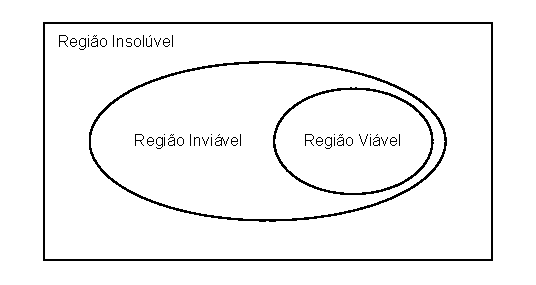
\includegraphics[scale=1.7]{textuais/capitulo1/figuras/regioes_seguranca.pdf}
    \label{fig:regiões de solução}
    \caption*{Fonte: Adaptada de Overbye (\citeyear{Overbye})}
\end{figure}


\begin{itemize}
    \item Região Viável: Região onde há solução para o problema que não viole os limites operacionais dos componentes do sistema;
    \item Região Inviável: Região onde há solução para o problema que viole um ou mais limites operacionais;
    \item Região Insolúvel: Região onde não há solução para o problema, onde provavelmente operar nessas condições geraria uma instabilidade que culminaria no colapso de tensão do sistema.
\end{itemize}

Estender a fronteira entre a região inviável e insolúvel oferece diversos benefícios principalmente no estudo de planejamento da expansão do \ac{SEP} e análise de contingências. Obter uma solução, mesmo inviável, pode facilitar estimativas de futuros projetos capazes de enfrentar um aumento de carga planejado, por exemplo.

Este estudo tem como motivação testar e analisar um método proposto por Iwamoto (1981)  que visa otimizar a atualização das variáveis de estado dentro do método de \ac{NR} e compará-lo com os métodos tradicionais em coordenadas polares e retangulares, visando explorar sua implementação. Isso envolve a análise teórica, o desenvolvimento de algoritmos computacionais e a realização de estudos de caso em sistemas de teste representativos.

\section{OBJETIVOS}
O objetivo deste trabalho consiste em fazer uma revisão bibliográfica acerca do método conhecido na literatura como Fluxo de Potência com Multiplicar Ótimo. Para isso, o trabalho foi dividido nas seguintes etapas:
\begin{itemize}
    \item Implementar o \ac{FPPOL} e \ac{FPRET};
    \item Implementar o \ac{FPMO};
    \item Testar e comparar os algoritmos em sistemas teste;
    \item Avaliar a utilização do método proposto explorando sistemas extremamente carregados, mapas fractais das múltiplas soluções do fluxo de potência e tempo computacional.
\end{itemize}

\section{ESTRUTURA DO DOCUMENTO}
A divisão deste trabalho é feita em cinco capítulos. O primeiro, de introdução, visa contextualizar e justificar ao leitor a necessidade da atual pesquisa, bem como definir os objetivos e a metodologia utilizada para o trabalho.

No capítulo 2, é feita uma revisão dos conceitos principais do \ac{FP} necessários para a compreensão adequada do tema, apresentando todo o desenvolvimento matemático, desde as séries de Taylor, até a formulação do método de \ac{NR} para ambos os sistemas de coordenadas retangulares e polares.

O capítulo 3 é composto pela formulação matemática completa do \ac{FPMO}, visando resolver os principais problemas encontrados ao tentar implementar o algoritmo.

O capítulo 4 será composto pelos resultados das simulações realizadas em sistemas teste, que servirão de apoio para as comparações dos métodos analisados.

Por último, o capítulo 5 engloba as conclusões finais alcançadas com o trabalho, somado de um futuro direcionamento para pesquisas posteriores.

